% Kazuki: results for Detail window (LTTB) and brief Event list note.

\section{Results}

Figure~\ref{fig:lttb} shows the LTTB comparison. With a budget of 300 points, LTTB tracks the
spikes of the dense reference, whereas stride at the same budget misses the tallest peak
(maximum 1874 counts with LTTB versus 1347 with stride in this example). LTTB is therefore
the default detail downsampler.

\begin{figure}[ht]
  \centering
  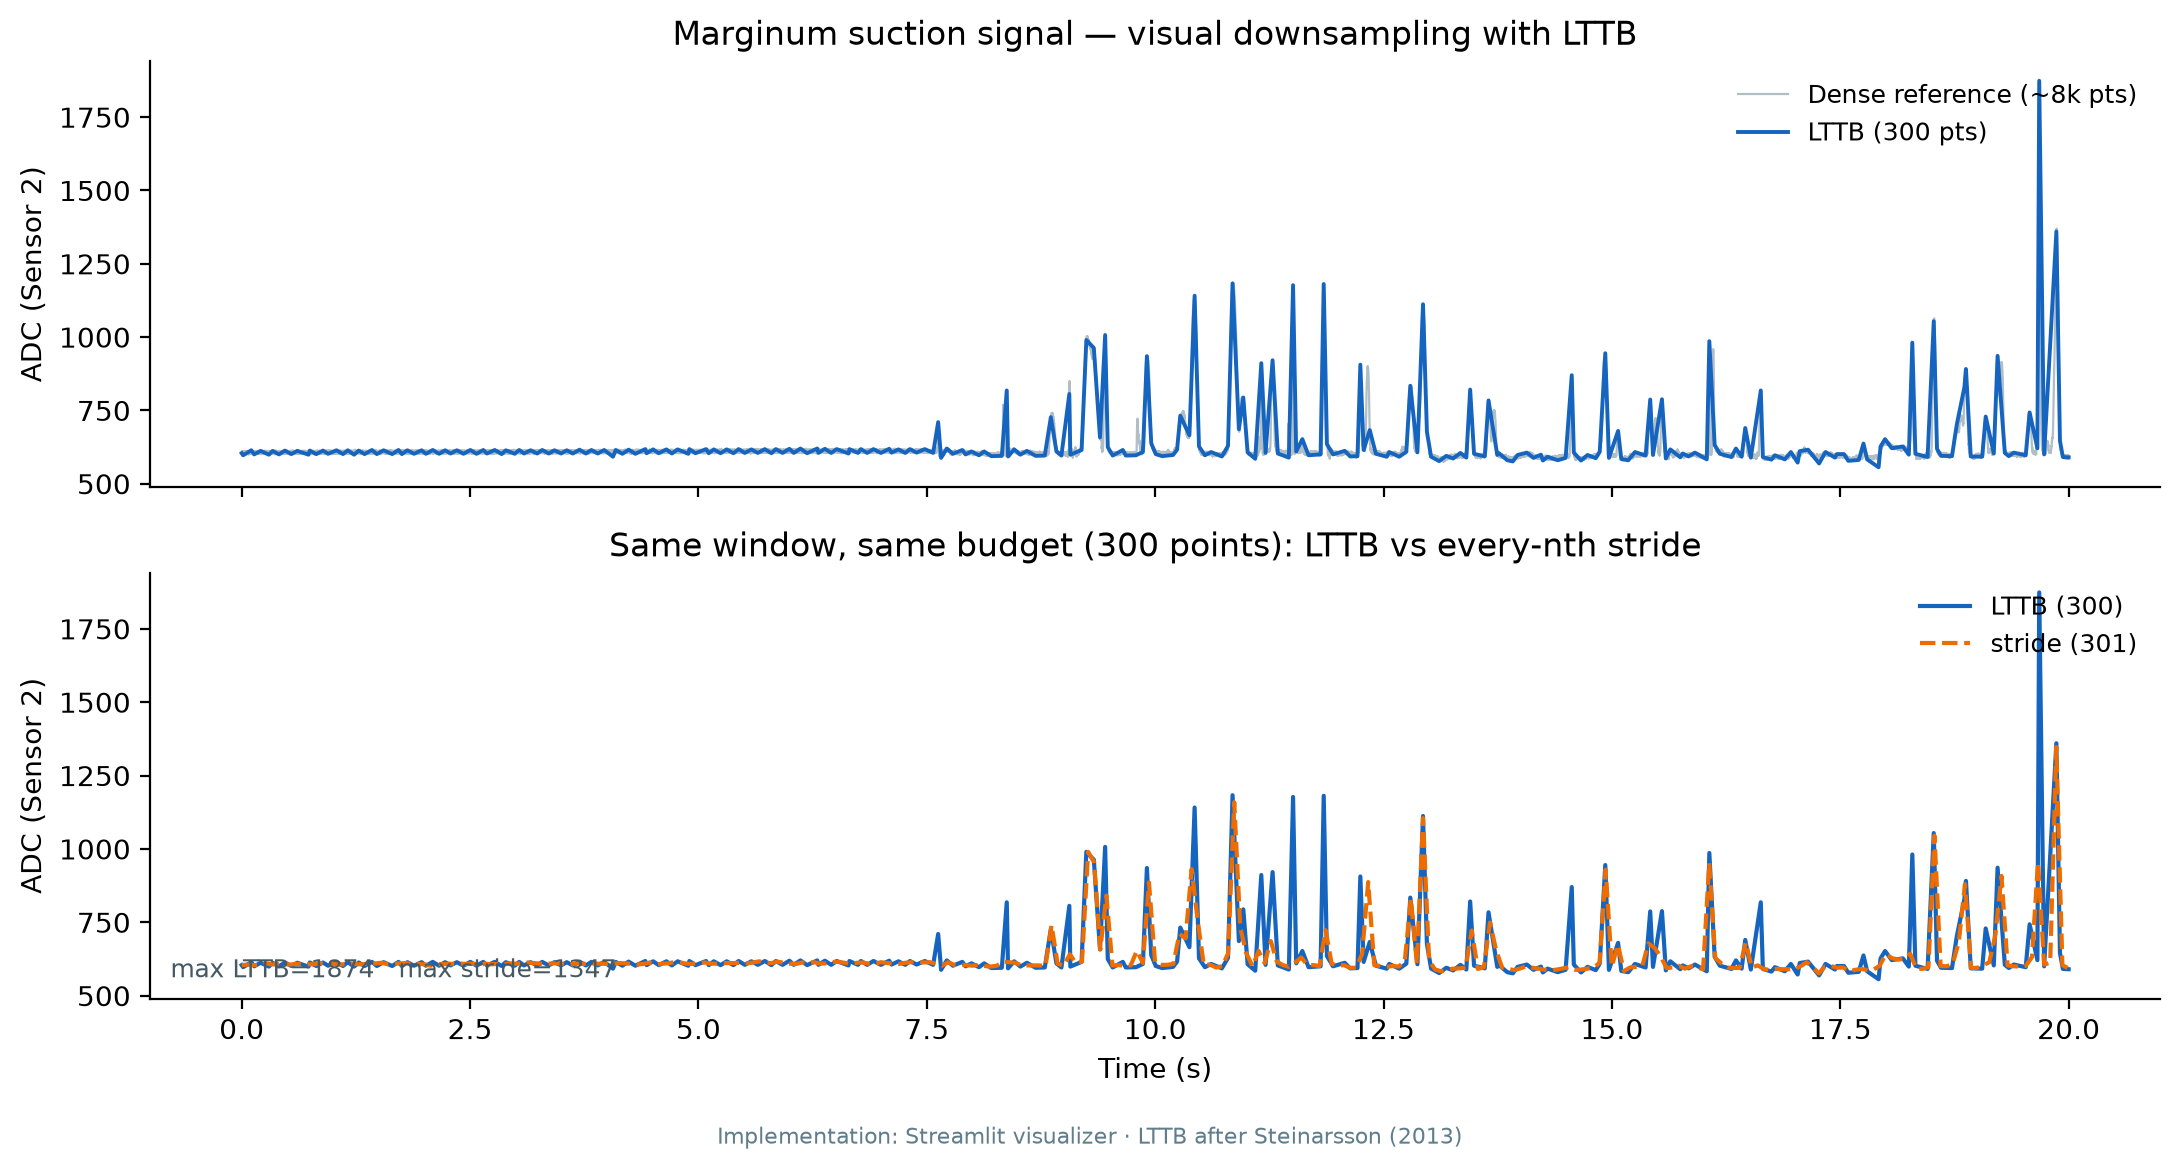
\includegraphics[width=\textwidth]{figures/lttb_marginum_visualization.png}
  \caption{Marginum suction signal (Sensor~2): LTTB versus a dense reference (top) and versus
  every-$n$th stride at the same 300-point budget (bottom), after
  Steinarsson~\cite{steinarsson2013}.}
  \label{fig:lttb}
\end{figure}

Selecting an event in the event list moves the detail window to that piece; the selected
event card updates to the corresponding label and peak time.
